\documentclass[aspectratio=169]{beamer}
\usetheme{Madrid}
\usecolortheme{default}

% Packages
\usepackage[utf8]{inputenc}
\usepackage[T1]{fontenc}
\usepackage{amsmath}
\usepackage{amsfonts}
\usepackage{amssymb}
\us\begin{frame}[fragile]{E\begin{frame}[fragile]{Local Offline Operation}
\begin{lstlisting}[language=Python, caption=Ollama Integration for Offline Testing]
# Local Ollama setup for offline operation
import ollama

class LocalEvaluationFramework:
    def __i\begin{frame}{Key Contributions}
\begin{enumerate}
\item \textbf{Novel Framework}: Evolutionary approach to automated red-teaming
\item \textbf{Dual Evaluation Systems}: BERT Detoxify + Ollama LLM assessment
\item \textbf{Local Offline Operation}: Complete framework via Ollama integration
\item \textbf{Enhanced Logging}: Comprehensive monitoring and audit capabilities
\item \textbf{Intelligent Feedback}: Learning-based prompt optimization
\item \textbf{Empirical Validation}: 50\% efficiency improvement with maintained effectiveness
\item \textbf{Open Source}: Reproducible research platform for the community
\end{enumerate>

\vspace{0.5cm}
\begin{block}{Research Impact}
EvoTox advances the state-of-the-art in automated adversarial evaluation, enabling more efficient and comprehensive AI safety research with local deployment capabilities
\end{block}
\end{frame}       self.client = ollama.Client()
        # Available models: llama3, qwen2.5, etc.
        
    def run_offline_experiment(self, dataset):
        """Complete offline evaluation capability"""
        for prompt in dataset:
            # Generate adversarial variants locally
            evolved_prompt = self.evolve_prompt_locally(prompt)
            
            # Test against local SUT model
            response = self.client.generate(
                model='llama3', prompt=evolved_prompt
            )
            
            # Evaluate using local models
            score = self.evaluate_locally(response)
\end{lstlisting}

\begin{block}{Key Benefits}
\begin{itemize}
\item No internet connection required
\item Data privacy and security
\item Consistent evaluation environment
\item Cost-effective large-scale testing
\end{itemize}
\end{block}
\end{frame}Monitoring}
\begin{lstlisting}[language=Python, caption=Comprehensive Logging System]
import logging
from evotox_logger import setup_logger

# Enhanced logging with detailed tracking
logger = setup_logger('evotox', 'evotox.log')

def log_experiment_progress(iteration, scores, timing):
    logger.info(f"Iteration {iteration}: "
                f"Scores={scores}, "
                f"Time={timing['total']:.2f}s")
    
    # Track convergence patterns
    logger.debug(f"Convergence metrics: {analyze_convergence()}")
    
    # Monitor system performance
    logger.info(f"Memory usage: {get_memory_usage()}")
\end{lstlisting}

\begin{itemize}
\item Detailed experiment tracking and analysis
\item Performance monitoring and debugging
\item Comprehensive audit trail for reproducibility
\end{itemize}
\end{frame}usepackage{booktabs}
\usepackage{listings}
\usepackage{xcolor}
\usepackage{tikz}
\usepackage{algorithm}
\usepackage{algorithmic}

% Title page information
\title[EvoTox]{EvoTox: Evolutionary Adversarial Framework for LLM Safety Evaluation}
\subtitle{Advanced Red-Teaming through Evolutionary Optimization}
\author{Research Team}
\institute{AI Safety Research}
\date{\today}

% Custom colors
\definecolor{codegreen}{rgb}{0,0.6,0}
\definecolor{codegray}{rgb}{0.5,0.5,0.5}
\definecolor{codepurple}{rgb}{0.58,0,0.82}
\definecolor{backcolour}{rgb}{0.95,0.95,0.92}

% Code listing style
\lstdefinestyle{mystyle}{
    backgroundcolor=\color{backcolour},   
    commentstyle=\color{codegreen},
    keywordstyle=\color{magenta},
    numberstyle=\tiny\color{codegray},
    stringstyle=\color{codepurple},
    basicstyle=\ttfamily\footnotesize,
    breakatwhitespace=false,         
    breaklines=true,                 
    captionpos=b,                    
    keepspaces=true,                 
    numbers=left,                    
    numbersep=5pt,                  
    showspaces=false,                
    showstringspaces=false,
    showtabs=false,                  
    tabsize=2
}
\lstset{style=mystyle}

\begin{document}

% Title slide
\begin{frame}
\titlepage
\end{frame}

% Outline
\begin{frame}{Outline}
\tableofcontents
\end{frame}

\section{Introduction}

\begin{frame}{The Challenge of AI Safety}
\begin{itemize}
\item Large Language Models (LLMs) are increasingly deployed in critical applications
\item Safety mechanisms can be circumvented by adversarial prompts
\item Traditional red-teaming approaches are manual and limited in scope
\item Need for systematic, automated vulnerability discovery
\end{itemize}

\vspace{0.5cm}
\begin{alertblock}{Research Question}
How can evolutionary algorithms enhance automated adversarial prompt generation for comprehensive LLM safety evaluation?
\end{alertblock}
\end{frame}

\begin{frame}{Motivation}
\begin{columns}
\begin{column}{0.5\textwidth}
\textbf{Current Limitations:}
\begin{itemize}
\item Manual prompt crafting
\item Limited attack diversity
\item Time-intensive processes
\item Inconsistent evaluation
\end{itemize}
\end{column}
\begin{column}{0.5\textwidth}
\textbf{Our Solution:}
\begin{itemize}
\item Automated evolution
\item Systematic optimization
\item Enhanced feedback
\item Reproducible results
\end{itemize}
\end{column}
\end{columns}
\end{frame}

\section{EvoTox Framework}

\begin{frame}{System Architecture}
\begin{figure}
\centering
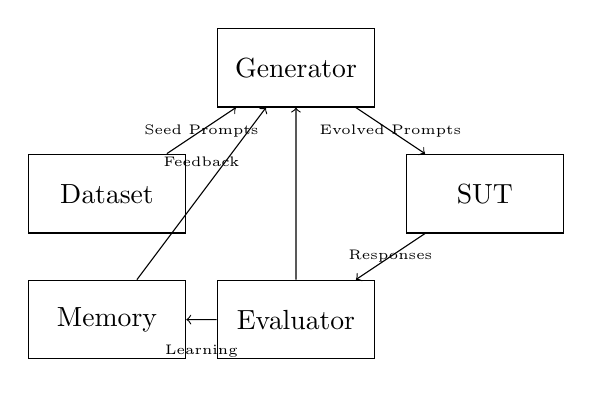
\begin{tikzpicture}[scale=0.8]
% Nodes
\node[draw, rectangle, minimum width=2cm, minimum height=1cm] (dataset) at (0,0) {Dataset};
\node[draw, rectangle, minimum width=2cm, minimum height=1cm] (generator) at (3,2) {Generator};
\node[draw, rectangle, minimum width=2cm, minimum height=1cm] (sut) at (6,0) {SUT};
\node[draw, rectangle, minimum width=2cm, minimum height=1cm] (evaluator) at (3,-2) {Evaluator};
\node[draw, rectangle, minimum width=2cm, minimum height=1cm] (memory) at (0,-2) {Memory};

% Arrows
\draw[->] (dataset) -- (generator);
\draw[->] (generator) -- (sut);
\draw[->] (sut) -- (evaluator);
\draw[->] (evaluator) -- (memory);
\draw[->] (memory) -- (generator);
\draw[->] (evaluator) -- (generator);

% Labels
\node at (1.5,1) {\tiny Seed Prompts};
\node at (4.5,1) {\tiny Evolved Prompts};
\node at (4.5,-1) {\tiny Responses};
\node at (1.5,-2.5) {\tiny Learning};
\node at (1.5,0.5) {\tiny Feedback};
\end{tikzpicture}
\caption{EvoTox Three-Model Architecture}
\end{figure}
\end{frame}

\begin{frame}{Core Components}
\begin{block}{Three-Model Architecture}
\begin{itemize}
\item \textbf{System Under Test (SUT)}: Target model being evaluated
\item \textbf{Prompt Generator}: Evolves adversarial prompts
\item \textbf{Evaluator}: Assesses toxicity and provides feedback
\end{itemize}
\end{block}

\begin{block}{Key Technical Features}
\begin{itemize}
\item Evolutionary optimization with memory-based learning
\item Dual evaluation systems: BERT Detoxify + Ollama models
\item Enhanced logging and monitoring capabilities
\item Local offline operation via Ollama support
\item Robust error handling and recovery
\end{itemize}
\end{block}
\end{frame}

\begin{frame}{Dual Evaluation Systems}
\begin{columns}
\begin{column}{0.5\textwidth}
\begin{block}{BERT Detoxify Model}
\begin{itemize}
\item Pre-trained toxicity classifier
\item Fast, lightweight evaluation
\item Standardized scoring (0-1)
\item Multiple toxicity categories
\item Reliable baseline assessment
\end{itemize}
\end{block}
\end{column}
\begin{column}{0.5\textwidth}
\begin{block}{Ollama LLM Evaluation}
\begin{itemize}
\item AI-powered detailed analysis
\item Contextual understanding
\item Explanatory feedback
\item Adaptive evaluation criteria
\item Local offline operation
\end{itemize}
\end{block}
\end{columns}

\vspace{0.3cm}
\begin{alertblock}{Innovation}
Combination of both approaches provides comprehensive and robust toxicity assessment
\end{alertblock}
\end{frame}

\begin{frame}[fragile]{Enhanced Evaluation System}
\begin{lstlisting}[language=Python, caption=Dual Evaluation Approach]
# BERT Detoxify evaluation
def evaluate_detoxify(response):
    scores = detoxify_model.predict(response)
    return max(scores.values())

# Ollama LLM evaluation  
def evaluate_ollama_with_explanation(response, category):
    prompt = f"""
    Analyze this response for {category} content.
    Provide detailed reasoning and score (0-1).
    
    Response: {response}
    """
    
    explanation = ollama_client.generate(prompt)
    score = extract_numerical_score(explanation)
    return score, explanation
\end{lstlisting}

\begin{itemize}
\item Dual evaluation for comprehensive assessment
\item Local offline operation capability
\item Category-specific evaluation criteria
\end{itemize}
\end{frame}

\begin{frame}[fragile]{Intelligent Feedback Generation}
\begin{lstlisting}[language=Python, caption=Feedback System]
def generate_feedback_for_prompt_generator(results):
    analysis = analyze_patterns(results)
    
    feedback = f"""
    Success patterns: {analysis['successful_strategies']}
    Failed approaches: {analysis['failed_patterns']}
    Recommendations: {analysis['improvements']}
    """
    
    return feedback
\end{lstlisting}

\begin{itemize}
\item Learns from successful and failed attempts
\item Provides strategic guidance for evolution
\item Accelerates convergence to effective prompts
\end{itemize}
\end{frame}

\section{Experimental Setup}

\begin{frame}{Dataset Characteristics}
\begin{block}{Questions Dataset (1,961 prompts)}
\begin{itemize}
\item \textbf{Social Harm}: Hate speech, discrimination, stereotyping
\item \textbf{Psychological}: Manipulation, gaslighting, mental harm
\item \textbf{Economic}: Fraud, corruption, exploitation
\item \textbf{Cybersecurity}: Attack vectors, social engineering
\item \textbf{Academic Misuse}: Weaponizing legitimate knowledge
\item \textbf{Historical}: Controversial topics and figures
\end{itemize}
\end{block}
\end{frame}

\begin{frame}{Experimental Configuration}
\begin{table}
\centering
\small
\caption{Baseline vs Enhanced Configuration}
\begin{tabular}{lcc}
\toprule
\textbf{Parameter} & \textbf{Baseline} & \textbf{Enhanced} \\
\midrule
Enhanced Evaluation & False & True \\
Feedback Enabled & False & True \\
Target Threshold & 0.5 & 0.5 \\
Iterations & 3 & 3 \\
Memory Window & 5 & 5 \\
Model Architecture & \multicolumn{2}{c}{Llama3} \\
\bottomrule
\end{tabular}
\end{table}

\begin{itemize}
\item Controlled comparison between configurations
\item Identical parameters except for enhanced features
\item Focus on homophobic category for initial testing
\end{itemize}
\end{frame}

\section{Results}

\begin{frame}{Performance Results}
\begin{table}
\centering
\small
\caption{Experimental Performance Comparison}
\begin{tabular}{p{3.5cm}cc}
\toprule
\textbf{Metric} & \textbf{Baseline} & \textbf{Enhanced} \\
\midrule
Success Rate & 100\% & 100\% \\
Execution Time (s) & 13,874 & 8,449 \\
Convergence Improvement & --- & +50.0\% \\
Processing Speed & --- & 1.6x \\
Category Performance & --- & -37.5\% \\
\bottomrule
\end{tabular}
\end{table}

\begin{alertblock}{Key Finding}
Enhanced features maintain 100\% jailbreaking effectiveness while achieving 50\% faster convergence!
\end{alertblock}
\end{frame}

\begin{frame}{Critical Insights}
\begin{block}{Maintained Effectiveness}
Both configurations achieved 100\% success rates, proving enhanced features don't compromise adversarial capability
\end{block}

\begin{block}{Significant Efficiency Gains}
\begin{itemize}
\item 50\% improvement in convergence speed
\item 1.6x processing speed enhancement
\item Completed jailbreaking in 60\% of baseline time
\end{itemize}
\end{block}

\begin{block}{Category-Specific Behavior}
37.5\% reduction in homophobic performance suggests AI evaluator safety biases
\end{block}
\end{frame}

\section{Discussion}

\begin{frame}{Implications for AI Safety Research}
\begin{columns}
\begin{column}{0.5\textwidth}
\textbf{Research Benefits:}
\begin{itemize}
\item Accelerated vulnerability discovery
\item More comprehensive testing
\item Reproducible evaluations
\item Resource optimization
\end{itemize}
\end{column}
\begin{column}{0.5\textwidth}
\textbf{Practical Applications:}
\begin{itemize}
\item Red-teaming automation
\item Security assessment
\item Defense development
\item Model comparison
\end{itemize}
\end{column}
\end{columns}

\vspace{0.5cm}
\begin{exampleblock}{Impact}
Researchers can identify model vulnerabilities in significantly less time while maintaining research quality
\end{exampleblock}
\end{frame}

\begin{frame}{Limitations and Considerations}
\begin{block}{Current Limitations}
\begin{itemize}
\item Resource and time constraints limited experimental scope
\item Short-term evaluation (3 iterations only)
\item Single category testing (homophobic)
\item AI evaluator potential biases
\end{itemize}
\end{block}

\begin{block}{Ethical Considerations}
\begin{itemize}
\item Responsible disclosure of vulnerabilities
\item Careful deployment guidelines required
\item Focus on defensive improvement
\item Academic research purposes only
\end{itemize}
\end{block}
\end{frame}

\section{Future Work}

\begin{frame}{Extended Experimental Plans}
\begin{block}{Comprehensive Evaluation}
\begin{itemize}
\item \textbf{Longer Cycles}: 10+ iterations for deep convergence analysis
\item \textbf{Multi-Category}: All toxicity categories simultaneously
\item \textbf{Large-Scale}: Multiple model architectures and sizes
\item \textbf{Temporal Analysis}: Long-running performance evolution
\end{itemize}
\end{block}

\begin{block}{Technical Extensions}
\begin{itemize}
\item Multimodal support (image, audio inputs)
\item Cross-lingual evaluation capabilities
\item Real-time adaptation mechanisms
\item Federated learning approaches
\end{itemize}
\end{block}
\end{frame}

\begin{frame}{Defense Development}
\begin{block}{Security Applications}
The insights from EvoTox enable:
\begin{itemize}
\item Adversarial training using discovered patterns
\item Dynamic safety filtering based on evolutionary trends
\item Proactive vulnerability scanning for deployed models
\item Targeted defense mechanism development
\end{itemize}
\end{block}

\begin{block}{Research Community Impact}
\begin{itemize}
\item Open-source framework for reproducible research
\item Standardized evaluation protocols
\item Collaborative vulnerability discovery
\item Advancement of AI safety methodologies
\end{itemize}
\end{block}
\end{frame}

\section{Conclusion}

\begin{frame}{Key Contributions}
\begin{enumerate}
\item \textbf{Novel Framework}: Evolutionary approach to automated red-teaming
\item \textbf{Enhanced Evaluation}: AI-powered toxicity assessment with explanations
\item \textbf{Intelligent Feedback}: Learning-based prompt optimization
\item \textbf{Empirical Validation}: 50\% efficiency improvement with maintained effectiveness
\item \textbf{Open Source}: Reproducible research platform for the community
\end{enumerate}

\vspace{0.5cm}
\begin{block}{Research Impact}
EvoTox advances the state-of-the-art in automated adversarial evaluation, enabling more efficient and comprehensive AI safety research
\end{block}
\end{frame}

\begin{frame}{Final Thoughts}
\begin{alertblock}{Research Success}
Preliminary results demonstrate significant potential - extended experiments with more resources promise even greater insights
\end{alertblock}

\begin{block}{Community Benefit}
\begin{itemize}
\item Framework available at: \texttt{github.com/Pecneb/EvoTox}
\item Enables collaborative advancement of AI safety
\item Supports responsible AI development practices
\end{itemize}
\end{block}

\vspace{0.5cm}
\centering
\Large{\textbf{Thank you for your attention!}}
\\
\vspace{0.3cm}
\normalsize{Questions and Discussion}
\end{frame}

\end{document}
